\graphicspath{{introduction/fig/}}

\chapter{Introduction}
\label{chap:introduction}

\section{Background}
In the modern world robots have become an integral part of our daily lives and society. For example the Xiaomi cleaning robot which can automatically clean a house floor.
Generally in robotics a manipulator (eg.
an arm) is used to manipulate an object in
the environment.

It is easier to first simulate the robots behavior in a
more simple environment which is why we will solve a similar and smaller problem as a step to a complete solution. By doing so we can save expenses, as it is costly to test a robot in reality while simulation is much cheaper. \newline

The sliding puzzle is a game with a history dating back to the 1870's. The aim of the game is to arrange a shuffled set of numbered tiles into ascending order by sliding and swapping the black/blank tile piece into one of its neighboring tiles. An example of a puzzle being solved is shown in \ref{fig:sliding_puzzle_figs}.

\begin{figure}[!htb]
	\centering
	\begin{subfigure}{.2\textwidth}
		\centering
		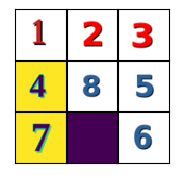
\includegraphics[width=.75\linewidth]{game_states/31.png}
		\caption{1a}
		\label{fig:sfig1}
	\end{subfigure}%
	\begin{subfigure}{.2\textwidth}
		\centering
		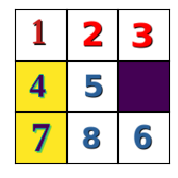
\includegraphics[width=.75\linewidth]{game_states/32.png}
		\caption{1b}
		\label{fig:sfig2}
	\end{subfigure}
	\begin{subfigure}{.2\textwidth}
		\centering
		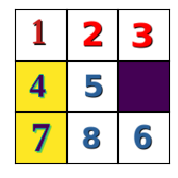
\includegraphics[width=.75\linewidth]{game_states/33.png}
		\caption{1b}
		\label{fig:sfig3}
	\end{subfigure}
	\begin{subfigure}{.2\textwidth}
		\centering
		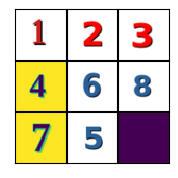
\includegraphics[width=.75\linewidth]{game_states/34.png}
		\caption{1b}
		\label{fig:sfig4}
	\end{subfigure}
	\caption{Figures of a 3x3 sliding puzzle being solved}
	\label{fig:sliding_puzzle_figs}
\end{figure}

\section{Problem Statement/ Research Aim}
In this project
we solve sliding puzzles using
reinforcement learning, where the same algorithm can then later be applied to the robotics problem of moving in an environment.

\section{Project Objectives}
\begin{itemize}
	\item Solve a 2x2 sliding puzzle using Reinforcement learning
	\item Solve a 3x3 puzzle using Reinforcement learning
	\item Puzzles must solve in a reasonable amount of time
\end{itemize}

\section{Scope}
Although there are many methods to solve a problem in RL, in this project we only look at two methods. These are SARSA (State-Action-Reward-State-Action) and Q-learning. 

Typically for problems with large state spaces, neural networks are used in conjunction with Reinforcement Learning techniques to save computational time. However for this project we will use a certain method to overcome the state space limitation which will be discussed later.

\section{Document Outline} 
Chapter \ref{chap:Literature_Review} looks at a paper which used an alternate approach to solve a 16 tile sliding puzzle.

Chapter \ref{chap:MDP_and_DP} describes in detail the mathematical background theory which forms the basis for Reinforcement Learning.

Chapter \ref{chap:RL} discusses in detail the Reinforcement Learning techniques which will be used to solve our puzzle problem.

Chapter \ref{chap:System_Design} lays out the overarching view of the software system, broken down into functional blocks.

Chapter \ref{chap:Experiments_and_Results} contains tests and verification that our solution works using the results of various experiments.

Chapter \ref{chap:conclusion} concludes the report.